% kernel.h — seven-pass pipeline diagram (TikZ).
% Mirrors the report's TikZ aesthetic (accent RGB{0,60,120}, rounded boxes,
% Stealth arrows). Rendered to a cropped PNG via pdflatex + pdftoppm + trim.
\documentclass[10pt]{article}
\usepackage[T1]{fontenc}
\usepackage[utf8]{inputenc}
\usepackage[margin=0cm]{geometry}
\pagestyle{empty}
\usepackage{xcolor}
\definecolor{accent}{RGB}{0,60,120}
\definecolor{codebg}{RGB}{248,248,248}
\usepackage{tikz}
\usetikzlibrary{arrows.meta,positioning}

\begin{document}
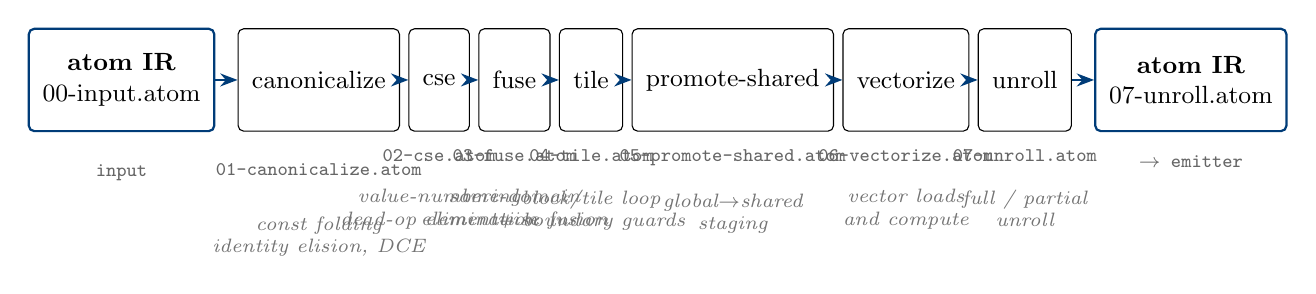
\begin{tikzpicture}[
  node distance=3pt,
  pbox/.style={draw, rounded corners=2pt, align=center, inner sep=5pt,
               fill=white, minimum height=1.3cm, font=\small},
  dbox/.style={draw, rounded corners=2pt, align=center, inner sep=4pt,
               fill=codebg, font=\footnotesize\ttfamily},
  iobox/.style={pbox, draw=accent, thick},
  parr/.style={-{Stealth[length=2.2mm]}, thick, draw=accent},
  dlbl/.style={font=\scriptsize\ttfamily, text=black!60, align=center},
  lbl/.style={font=\scriptsize\itshape, text=black!55, align=center},
]
  % ---- input ----
  \node[iobox] (in) {\textbf{atom IR}\\00-input.atom};

  % ---- the seven passes ----
  \node[pbox, right=8pt of in] (c1) {canonicalize};
  \node[pbox, right=of c1] (c2) {cse};
  \node[pbox, right=of c2] (c3) {fuse};
  \node[pbox, right=of c3] (c4) {tile};
  \node[pbox, right=of c4] (c5) {promote-shared};
  \node[pbox, right=of c5] (c6) {vectorize};
  \node[pbox, right=of c6] (c7) {unroll};

  % ---- input label ----
  \node[below=8pt of in, dlbl] (d0) {input};

  % ---- dump labels beneath each stage ----
  \node[below=8pt of c1, dlbl] (d1) {01-canonicalize.atom};
  \node[below=3pt of c2, dlbl] (d2) {02-cse.atom};
  \node[below=3pt of c3, dlbl] (d3) {03-fuse.atom};
  \node[below=3pt of c4, dlbl] (d4) {04-tile.atom};
  \node[below=3pt of c5, dlbl] (d5) {05-promote-shared.atom};
  \node[below=3pt of c6, dlbl] (d6) {06-vectorize.atom};
  \node[below=3pt of c7, dlbl] (d7) {07-unroll.atom};

  % ---- one-line description beneath each pass ----
  \node[below=8pt of d1, lbl] (s1) {const folding\\identity elision, DCE};
  \node[below=3pt of d2, lbl] (s2) {value-numbering\\dead-op elimination};
  \node[below=3pt of d3, lbl] (s3) {same-domain\\elementwise fusion};
  \node[below=3pt of d4, lbl] (s4) {block/tile loop\\+ boundary guards};
  \node[below=3pt of d5, lbl] (s5) {global$\to$shared\\staging};
  \node[below=3pt of d6, lbl] (s6) {vector loads\\and compute};
  \node[below=3pt of d7, lbl] (s7) {full / partial\\unroll};

  % ---- arrows between boxes ----
  \draw[parr] (in) -- (c1);
  \draw[parr] (c1) -- (c2);
  \draw[parr] (c2) -- (c3);
  \draw[parr] (c3) -- (c4);
  \draw[parr] (c4) -- (c5);
  \draw[parr] (c5) -- (c6);
  \draw[parr] (c6) -- (c7);

  % ---- output ----
  \node[iobox, right=8pt of c7] (out) {\textbf{atom IR}\\07-unroll.atom};
  \draw[parr] (c7) -- (out);
  \node[below=5pt of out, dlbl] {$\to$ emitter};
\end{tikzpicture}
\end{document}
